%!TeX encoding = UTF-8
%!TEX program = xelatex
% ============================================================
% 《X 射线晶体学》课程论文模板 —— LaTeX 版
% 源文档：X-Ray/课程资料/X-射线晶体学-课程论文模板.pdf
% 编译方式：XeLaTeX（连续两次），或运行本目录 complie.bat
% ============================================================
\documentclass[12pt,a4paper,twoside]{ctexart}

% ==================== 页面设置 ====================
\usepackage[top=2.4cm,bottom=2.5cm,left=1.5cm,right=1.4cm,footskip=0.55cm]{geometry}

% ==================== 字体（对照原模板：中文楷体、数字 Times New Roman）====================
\setCJKmainfont{KaiTi}[AutoFakeBold=2.0]
\setmainfont{Times New Roman}
\setlength{\parindent}{0pt}
\setlength{\parskip}{0pt}
\raggedbottom

% ==================== 颜色（取自原模板）====================
\usepackage{xcolor}
\definecolor{secblue}{HTML}{365F91}    % 一、二级标题蓝
\definecolor{subblue}{HTML}{243F60}    % 三级标题蓝
\definecolor{bandblue}{HTML}{9CB8C7}   % 首页标题色带

% ==================== 图表 ====================
\usepackage{graphicx}
\usepackage{float}
\usepackage{caption}
\DeclareCaptionFont{capfont}{\fontsize{8pt}{11pt}\selectfont}
\captionsetup{labelfont=normalfont,labelsep=space,font={capfont},justification=raggedright,singlelinecheck=false}

% ==================== 标题样式 ====================
\ctexset{
  section = {
    format     = {\color{secblue}\bfseries\fontsize{13pt}{16pt}\selectfont},
    number     = {\thesection.},
    aftername  = {\hspace{0.4em}},
    beforeskip = 15pt plus 3pt minus 2pt,
    afterskip  = 7pt plus 2pt,
  },
  subsection = {
    format     = {\color{secblue}\bfseries\fontsize{12pt}{15pt}\selectfont},
    aftername  = {\hspace{0.4em}},
    beforeskip = 12pt plus 2pt,
    afterskip  = 5pt plus 1pt,
  },
  subsubsection = {
    format     = {\color{subblue}\bfseries\fontsize{11pt}{14pt}\selectfont},
    aftername  = {\hspace{0.4em}},
    beforeskip = 10pt plus 2pt,
    afterskip  = 4pt plus 1pt,
  },
}

% ==================== 说明文字（原模板中的楷体小字，9.3pt）====================
\newcommand{\smtext}[1]{{\fontsize{9.3pt}{12pt}\selectfont #1}}

% ==================== 页脚（奇数页右下“| 页码”，偶数页左下“页码 |”）====================
\usepackage{fancyhdr}
\pagestyle{fancy}
\fancyhf{}
\renewcommand{\headrulewidth}{0pt}
\fancyfoot[RO]{\fontsize{8pt}{10pt}\selectfont |\enspace\thepage}
\fancyfoot[LE]{\fontsize{8pt}{10pt}\selectfont \thepage\enspace|}
\fancypagestyle{plain}{%
  \fancyhf{}%
  \renewcommand{\headrulewidth}{0pt}%
  \fancyfoot[RO]{\fontsize{8pt}{10pt}\selectfont |\enspace\thepage}%
}

\begin{document}
\linespread{1.0}\selectfont

% ==================== 首页题头 ====================
\hspace*{0.25cm}%
\begin{minipage}[c]{15.75cm}
  \setlength{\fboxsep}{0pt}%
  \colorbox{bandblue}{%
    \parbox[c][0.73cm][c]{15.75cm}{%
      \hspace{0.06cm}\textcolor{white}{\fontsize{16pt}{16pt}\selectfont\songti 《X 射线晶体学》课程论文}}}
\end{minipage}\hfill
\begin{minipage}[c]{1.4cm}
  \centering
\includegraphics[height=1.27cm]{assets/MUC.jpg}
\end{minipage}

\vspace{0.85cm}

\hspace*{3.9cm}{\songti\fontsize{12pt}{16pt}\selectfont 姓名，学号，班级}

\vspace{8pt}

\hspace*{3.9cm}{\songti\fontsize{8pt}{11pt}\selectfont 摘要\quad 简要介绍该论文的主要内容、意义（字数：200\textasciitilde300）}

% ==================== 1 引言 ====================
\section{引\hspace{0.5em}言}

\smtext{简要介绍X射线衍射的用途、意义。}

\smtext{【格式：论文章节1】}

\smtext{【格式：论文正文】}

% ==================== 2 晶体学基础 ====================
\section{晶体学基础}

\smtext{简要归纳晶体学的基础知识，如何描述晶体。}

\subsection{晶体的基本性质}

\subsection{晶体的描述}

\smtext{【格式：论文章节2】}

\subsubsection{原胞与晶胞}

\smtext{【格式：论文章节3】}

\subsubsection{对称性与空间群}

\subsubsection{晶胞内的原子}

\subsection{晶体的可视化}

\smtext{图文详细介绍利用diamond进行晶体建模的过程、注意事项。}

\subsubsection{利用Diamond软件建立晶体结构模型}

\subsubsection{常见晶体结构的特征}

% ==================== 3 X 射线衍射原理 ====================
\section{X射线衍射原理}

\subsection{X射线散射}

\subsubsection{原子对X射线的散射}

\subsubsection{晶体对X射线的散射}

\subsection{晶体衍射几何}

\subsubsection{布拉格方程}

\subsubsection{艾瓦德球与粉末衍射}

% ==================== 4 X-射线衍射仪 ====================
\section{X-射线衍射仪}

\smtext{简要介绍X-射线衍射仪的结构和功能，基本操作}

\subsection{X-射线衍射仪的结构}

\subsubsection{X射线的产生}

\subsubsection{X射线的探测}

\subsubsection{X射线衍射仪的仪器结构}

\subsection{X-射线衍射仪的操作}

\subsubsection{粉末衍射样品的制备}

\subsubsection{样品位置对衍射数据的影响}

\subsubsection{X射线衍射的实验技术}

% ==================== 5 X-射线衍射数据的基本处理 ====================
\section{X-射线衍射数据的基本处理}

\smtext{该部分侧重于对实验数据的表示（绘图）和数据的基本处理。}

\subsection{实验数据的表示}

\subsubsection{叠加有PDF卡片的XRD图绘制}

\smtext{衍射数据+PDF卡片的绘制}

\subsubsection{Rietveld晶体结构精修结果的绘制}

% ----- 插图示例（原模板中的示例图）-----
\begin{figure}[H]
  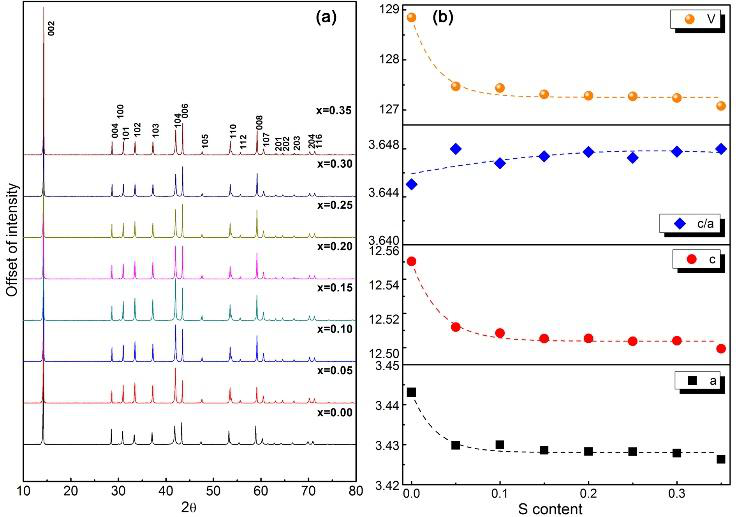
\includegraphics[width=8.5cm]{assets/example-xrd.png}
  \caption{……纳米材料的基本结构。(a) ……样品的XRD 图；(b)…}
  \label{fig:example}
\end{figure}

\smtext{每副图要有题注，每张表要有表头}

\subsection{数据的基本处理}

\smtext{数据处理的步骤，要点，注意事项}

\subsubsection{扣背底}

\subsubsection{平滑}

\subsubsection{寻峰}

\subsubsection{拟合}

% ==================== 6 常用 X 射线分析方法 ====================
\section{常用X射线分析方法}

\smtext{图文说明几种常用的X射线分析方法、注意事项}

\subsection{物相识别}

\subsubsection{物相识别原理}

\subsubsection{Mdi Jade中的物相识别}

\smtext{单一物相+多物相识别}

\subsection{仪器曲线的制作}

\subsubsection{角度校正曲线的校正}

\subsubsection{FWHM曲线的制作}

\subsection{定量物相分析}

\subsection{晶格参数的确定}

\subsubsection{指标化确定未知结构的已知结构}

\subsubsection{已知结构的晶格参数精修}

\subsubsection{制作自己的PDF卡片}

% ==================== 7 结论 ====================
\section{结\hspace{0.5em}论}

\smtext{简要总结上述各方法的用途和意义，简要归纳在这门课上学到了什么、还想学什么、对所学课程的建议。}

% ==================== 致谢 ====================
\section*{致\hspace{0.5em}谢}

\smtext{简要感谢在这门课学习中对自己有帮助的同学、老师的工作。}

% ==================== 参考文献 ====================
\section*{参考文献}

\smtext{文中所有不是由自己推导、分析得到的，而是从他人论文、出版物借用过来的，均需在正文部分用数字[1…]引用，在参考文献中按引用先后依次给出。}

\smtext{作者, 文章标题, 期刊名, (时间), 卷(期), 页码.}

\smtext{[1] Jeong IK, Heffner RH, Graf MJ and Billinge SJL, Lattice dynamics and correlated atomic motion from the atomic pair distribution function, Physical Review B, (2002), 67(10), 25-31.}

{\songti\fontsize{9.3pt}{12pt}\selectfont [2] 张代钧, 徐龙君, 用X射线径向分布函数法（RDF）研究煤中碳原子层的堆垛结构, 燃料化学学报, (1997), 25(4), 368-372.\par}

\end{document}
